\chapter{Foods We Ate}
Mere thought or mention of Thandi daal and garam prantha (cold lentils and
hot fried bread) awaken the senses of taste and smell amidst sounds of
a bustling happy family, with a clear picture of Mataji as the conductor
of the beautiful symphony played at 2, Model Town, Panipat, India in the
1950s and early 1960s. The hustle bustle, hugs and laughter add life to
the scene. 

It initiates mouth watering Pavlov's reflex and sliver of a water in the
eyes as the mind gets transported to those heavenly days.

Distinct visualisation of the multi-layered pranthe straight from the
tandoor, transports and merges us into the past of caring love and
a variety of perfectly prepared foods provided by our Pita Ji and
magically cooked by our mother, MataJi. They are voraciously consumed by
the fast growing jumping giggling bodies. 

Hearing the word or seeing Amrood (guava) or Dussehri mango brings forth
the images of young Pita Ji, ordering the best plants from the nursery and
getting them planted for the use of his growing family in 1950. The
greenery of plants and trees, the variety of fruits hanging from the
branches; the color and fragrance of the flowers surrounding the house
engulfed those who were fortunate to be part of this home. 

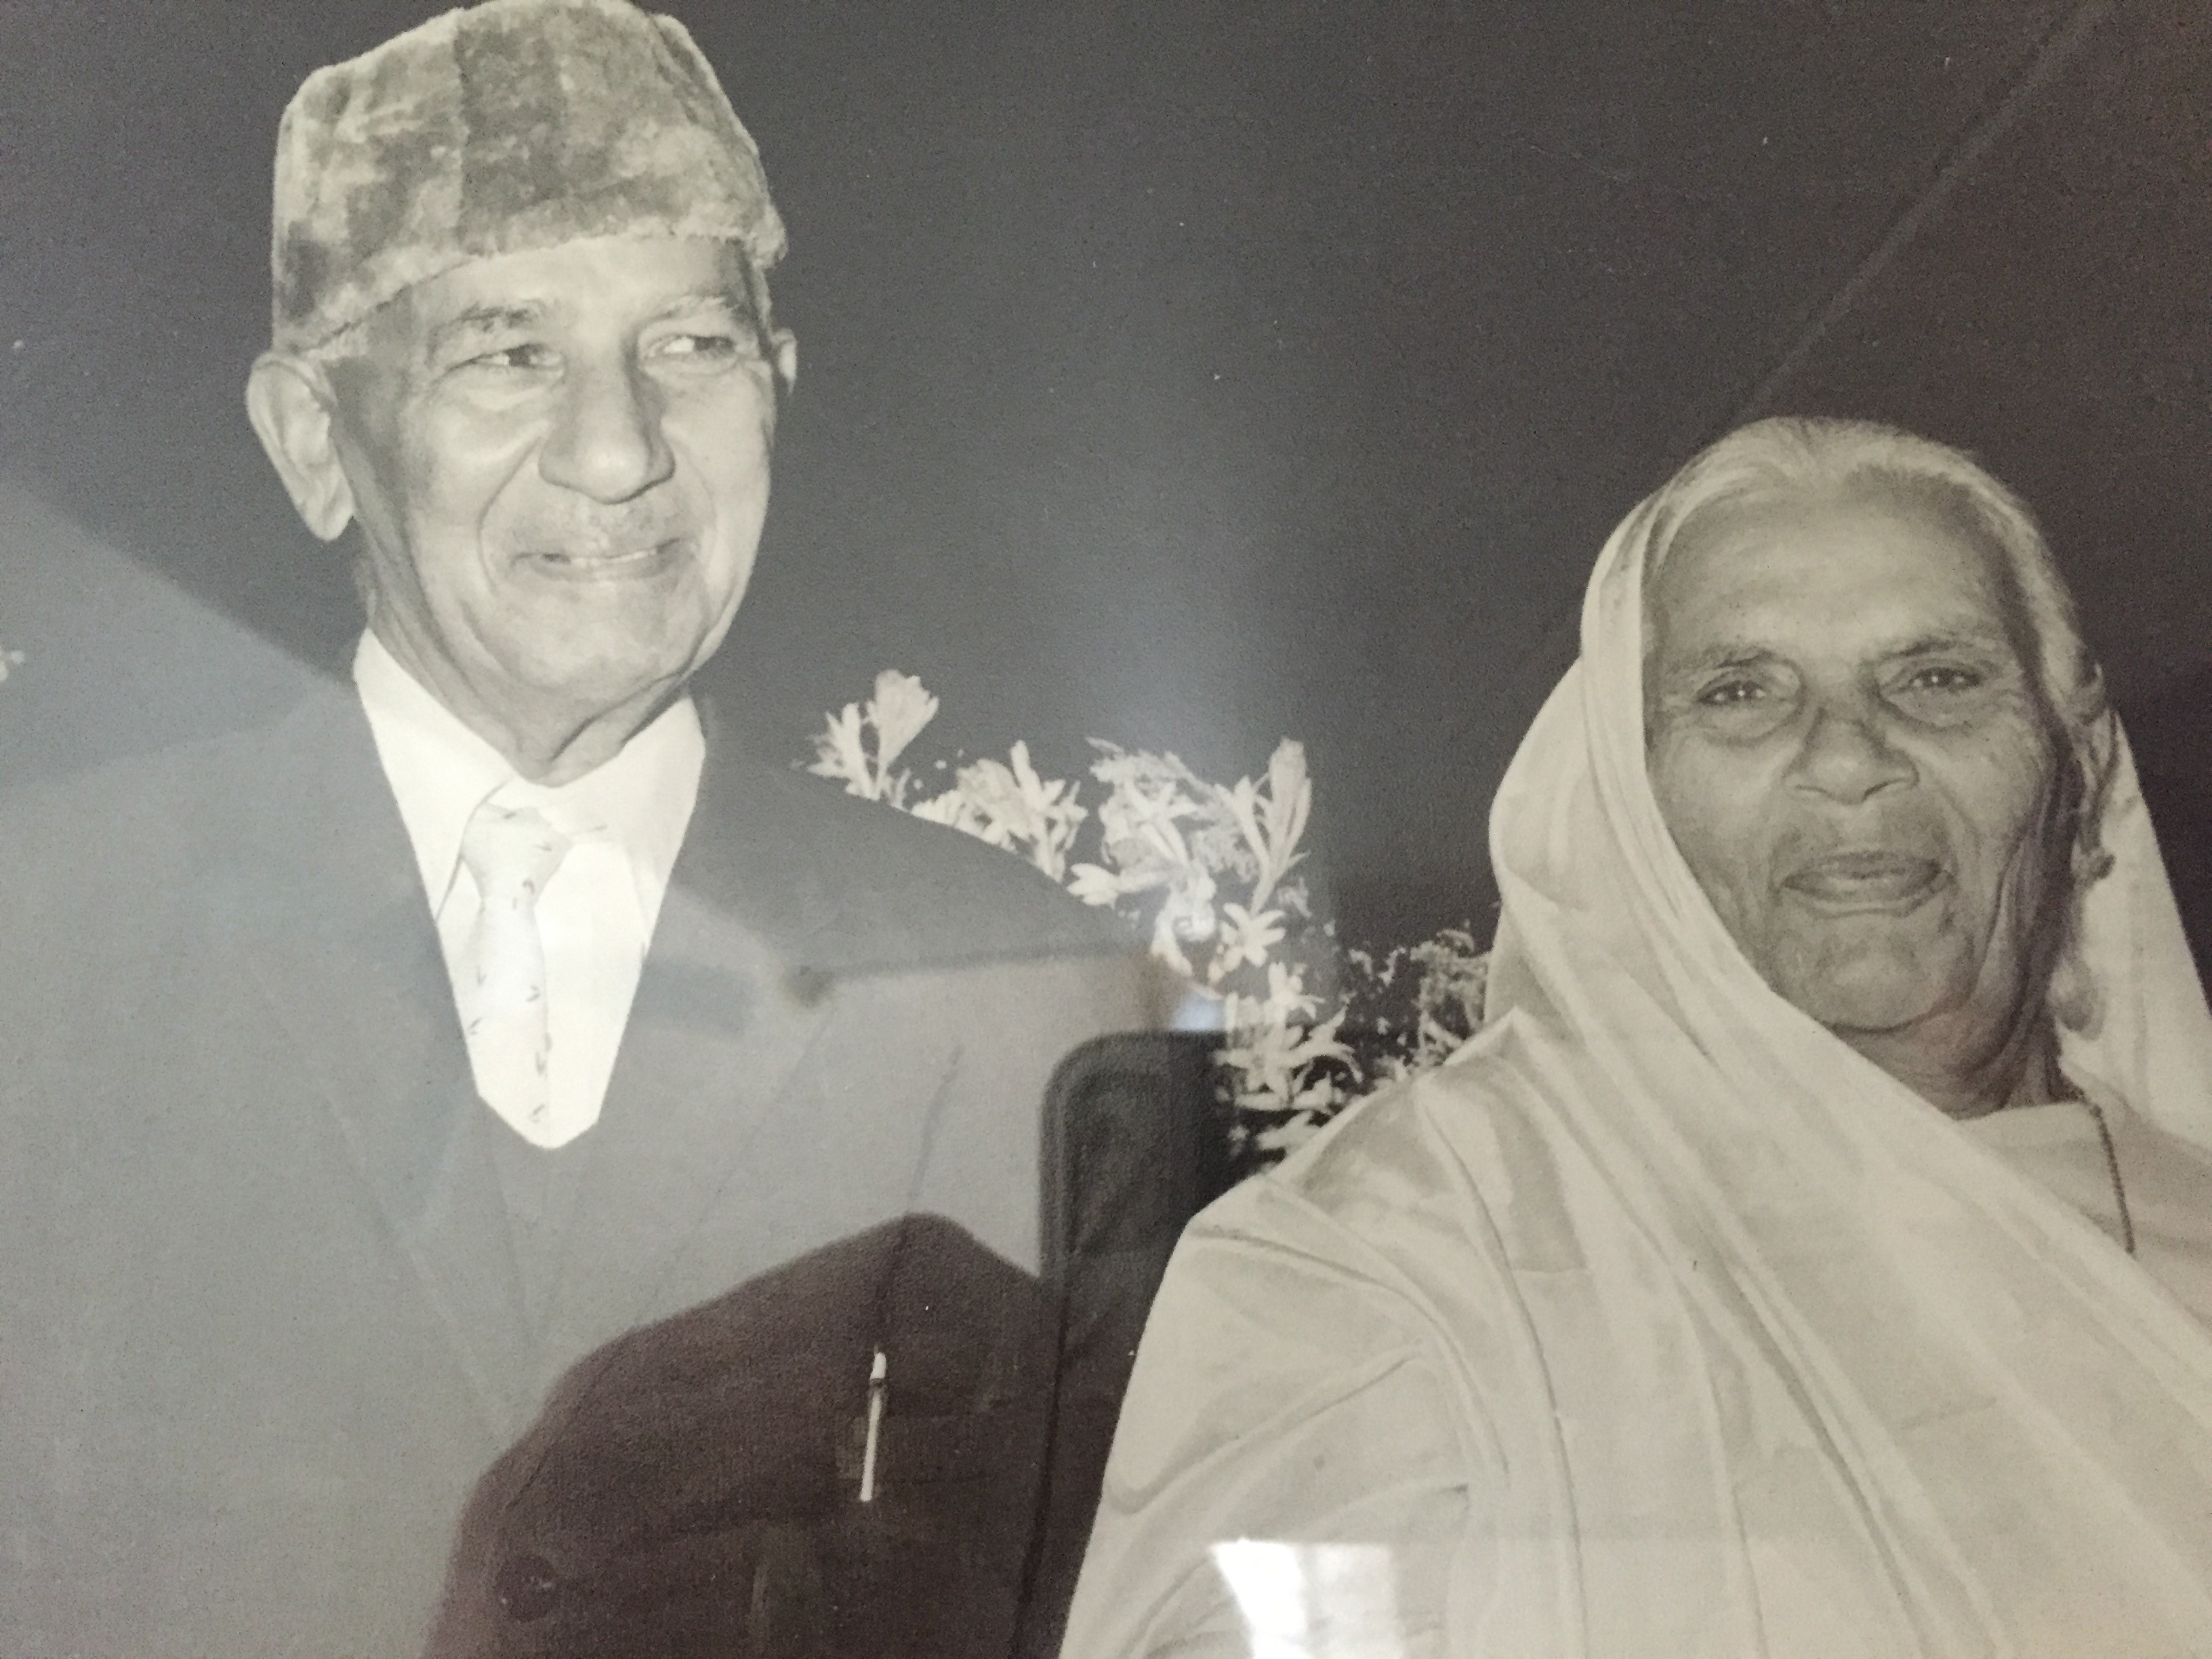
\includegraphics[width=.8\textwidth]{eating_pic_1.jpg}

The home-cooked food is painstakingly, always lovingly prepared and
generously served by Mataji. Home grown fruit trees and vegetable plants
are tenderly cared for by Pitaji and his little soldiers. Various
festivals, celebrations and frequent sprinkling of, mostly unannounced but
always welcome, guests brings in foods that are not commonly served. 

We are a large family and have limited resources; we are refugees as
a result of the recent partition of the country resulting in our migration
to the new land. Mataji is always working from 5 am to who knows when. She
is busy washing clothes, jharhoo poncha (brooming and dusting), but mostly
chopping vegetables, cooking and serving. 

By this time she is done being pregnant every other year, having given
birth to 10 children between 1928 to 1947. Two did not survive past the
age of five years, while we were still in that part of India which on
August 14, 1947 became known as West Pakistan. 

Pita Ji is mostly away from home procuring money by working at the newly
learnt job of making bricks at the out-of-town brick kilns. He supplements
the income by bringing home some and selling some of the produce from the
farm land allotted to him in partial reparation of several acres we were
forced to abandon in Pakistan. 

He is kind hearted and generous to a fault at his own expense. The
laborers at the farm are poorer than us. He gives away most of the produce
to the families of the labor. As a result, sometimes he gets an angry
response from Mataji who has been waiting for the vegetables. "Apne
bachche bhukhe so jaan pur tuhanu kee parvaah" (our children may sleep
hungry, but what do you care). He pleads, "Laborers have children too, who
will definitely go without any food without our help. We may be poor but
our children still have lot more.” He is right. We did feel the churning
stomach causing hunger pains but there is always something to eat. If
nothing, we just climb on a mango or guava tree and get fresh fruit. 

The days start with fried pranthas made on the skillet, home made yogurt,
sometimes cold black or yellow lentils (thandi daal) and achaar. One Anna
or dwanni (1/16 or 1/8 of a rupee) is our lunch money with which, during
school recess, we can buy food from the open stalls outside the school. 

After walking or running home from school we are given a steel glass full
of hot milk. Hectic outdoor playing requires much needed calories in the
form of vegetables and many wheat rotis during dinner. Night cap is
a glass of warm milk mixed with bread and sugar. On lucky days, it is
filled with jalebi. 

Almost everything is prepared from scratch. Wheat is the most commonly
used flour. Pitaji purchases large jute sacs filled with wheat kernels.
The wholesalers dusts the wheat with DDT to protect it from insects. No
one knew, till much later, that DDT was a risk factor in causing cancer,
when its use was banned. 

Small portions of wheat are placed in a flat tray made of bamboo strips
with its sides and back raised. It is gently shaken to get the husk
separated from the kernels. The husk is gently discarded by shaking the
tray, blowing it away or let the wind do the job. 

The boys partially fill the oval steel drum with water, drawn manually,
from the hand pump in the front yard. Using small buckets we put the
kernels into the water. Playfully, we swish the kernels around and
splashed water on one another. The faint dark water containing dust, DDT
and small floating bugs, called Ghun, is drained. Nothing is wasted. 

Narrow brick lined naaliyaan (channels) take the water to the thirsty
plants and trees. More water from the hand pump, more rinsing and draining
till the water looked clean, brings a cheerful relief. Shukar hai! 

White sheets are spread out on the cots or floor in the yard. We spread
out the kernels evenly for them to dry out in the hot sun which shines
over Panipat everyday except during the monsoon season. 

Our job is also to keep an eye on the ever hungry larks, doves, pigeons,
sparrows, crows and parrots. Beating steel drums with sticks to make loud
sound and shooting stones with our gulel (slingshot) keeps the invaders
away most of the time. 

Dry kernels are then placed in more manageable sacs or containers. Loaded
on the carrier of our prized bicycle, we pedal across the open fields into
a new development called 8 Marla with much smaller homes. Aate di Chakki
(flour mill) is owned by a kind, always smiling man. An electric motor
runs the flour mill. He puts kernels in the large opening at the top and
whole wheat flour comes out from the chute, a magical event to us.
Containers are refilled with ground wheat flour. We secure them on the
carrier and peddle our way home. Pitaji settles the bill every month. 

Prior to this machine we had a Chakki (Manual Grind) at home. This is made
of two round rough stones, with a minimal gap between them, stacked and
kept together by a vertical piece of wood going through a hole in the
center. The top one has a hole for feeding it with wheat kernels and
a vertical handle near the edge for rotating it. Rotating off the top
stone grinds the kernels between the two stones and aata spills out at the
edges. It is hard work. When one hand gets tired we switch hands and, to
catch our breath; all of us take turns. 

The flour is stored in air tight metal containers (peepe) with a hinged
lid that is latched securely. Even then it is not uncommon to see Susrian
(Weevils) crawling around in the flour. They are small black cylindrical
shaped bugs which find their way into the flour. Or most likely their eggs
hang on to the kernels, escape the effects of DDT or crushing and are now
happily hatching in the flour. No one freaks out; it is normal and just
another nuisance we learn to live with. We were not so rich to discard the
whole thing. Susrian are manually picked out or we use a fine chaanani
(sieve) to let the aata (flour) go through into a more secure container
and discard the susrian crawling around in the chaanani. Any remaking ones
or their Aggarwa are going to get cremated on the skillet anyway. 

In addition to the wheat we sometimes buy pre-made flour of barley or
corn. Combination of Makki di roti, makhkhan and saag (corn bread, butter
and spinach) is one of the classic Punjabi foods. Made out of corn flour,
the thick large roti cooked on skillet with slow heat or in the tandoor
till black spots start showing on the surface. A clump of home made butter
in the middle with a side dish of sarson da saag (mustard leaves) and
a glass of lassi (yogurt mixed with water and rock salt) is heavenly
combination for any Punjabi, anywhere. It is usually served for lunch,
which induced a deep slumber on a cot in the shade of a tree. 

Cooking is done indoors or outdoors depending on the weather. In early 50s
outdoor cooking is done on a clay 'Chulha'. It is a U shaped structure
hand made with clay at home. The approximately 2 inches thick walls were
about 10 inches high. The first chulha was placed near the southern
boundary wall of the house. Later on a gate was built in that section of
the wall and the chula was moved closer to the house, near the large mango
tree. 

For the purpose of creating cooking fire, the children gather dry tree
branches from the surrounding woods and stack them. We purchased larger
logs of wood from the market. 

A unique source of fuel is made from the cow dung called 'gobar'. We
follow a herd of stray cows with a round shallow metal container and
a scooper in our hands. Even though we close our noses, the large green
clumps are a delight to our eyes. We run to collect them in the container
till it is filled or too heavy to carry on our heads. The precious free
material is placed in a heap near the south boundary wall. It is mixed
with Toodhi (cut pieces of dry wheat plant). Round balls are flattened
with bare hands into a 8 to 10 inch round patties, called Goye, and stuck
to the walls. Hot sun dries them in a few days, at which time they are
peeled off and stacked in piles. They are excellent fuel for slow cooking
and perfect example of not letting even the animal waste go waste. 

Dry wood and goye are placed in the chulah through the open end of the U.
A fire is lit and air is blown into it through an about 18 inches long
metal cylindrical pipe called 'Phookni'. Dried ashes fly back making us
squint our eyes. Invariably some ashes and smoke get to the eyes. Watering
of the eyes is a common consequence of using phookni. Once the fire
starts, smoke vanishes and our natural stove is ready for the magic
through Mataji's hands. 

The flour is mixed with water and dough is kneaded (guniya)in a large
metal deep dish called praat. She makes round balls and by deftly slapping
them between two hand she creates a perfectly round roti. Tawa, metal
skillet, has already been heated on the flame. One after another,
countless rotis are cooked. The puffier the roti, the hungrier are the
eaters, is a common saying. 

A glob of home made butter or a half spoon of ghee is placed over the roti
and served hot on a steel plate. A burki (piece) from the roti is broken
off by fingers and used to wrap up one or two vegetables and eaten with
great delight and to no end, unless the Aata finishes. Onions and home
made achar are the condiments; or sometimes the only accompaniments of
rotis if there are no home grown vegetable or money. They are also common
dishes for Mataji, who unbeknown to us, keeps giving us the cooked
vegetables till there is nothing left for herself. 

All types of lentils are prepared. Udhad ki dal is most commonly made. It
is kept in a pot full of water and cooked on low heat for several hours.
Chane ki dal is notorious for producing noxious gases next day. In fact,
if someone farted with a foul smell, he was asked "Kal chole di daal khaai
see kya?"(Did you eat chick pea lentils yesterday?)

Sometimes Mataji grates cauliflower and/or white radish and uses them as
fillings to make pranthas. Garnished with butter, they are a delight to
eat with salted yogurt. Kali Daal is all time favorite for all. 

Some days she makes Choori for us. It is ghee filled roti broken up into
small pieces and has sprinkling of granulated jaggery or Shakkar. 

In October 2013, Prem, on a flying three days visit at Virinder and
Santosh's home in Delhi, had asked Salomi to make Choori for him. Such was
the impact of the loving and delicious food of our childhood and its
impressions on the hard drive of our brains. That was his last serving of
choori, he died at the age of 81 years in February 2014 

We also have an outdoor Tandoor in the corner between the walls of the
kitchen and small dining room, facing the north boundary wall. Tandoor is
an oval cylindrical structure made of clay. It is open on the top and
closed all around except for a small hole in the side wall near the
bottom. It let the air flow through while cooking and ashes out at the
end. 

It is preheated by burning wood logs and dried branches in it. Once the
wood has turned into red coal and the inside walls of tandoor take on
reddish hue, Mataji bravely inserts her hand carrying the round flat dough
(roti) on the front and a thick cloth for protection on the back. The
rotis are stuck to the hot wall. Once a young boy from Bombay, who had
never seen a tandoor, was visiting and was awed by the roti sticking to
the hot tandoor wall. He asked Mataji "Do you put glue on the roti before
sticking it to the wall?" 

One roti followed the other till the dough was finished. The cooked
tandoori rotis are snapped off by hand or a chimta (metal prong). 

Some of us love dry kadhak (crisp) roti while some love a generous ball of
butter or melted ghee. Mataji creates several variations to the basic
theme of the tandoori roti. Some are single layered, some multi-layered
with a coating of ghee between the leaves of dough; some sprinkled with
red mirchi or stuffed with onions or boiled mashed potatoes. Sometimes
rotis are made with the flour made from barley or corn. 

The family members sit on cots or chairs pulled out of the house. Thandi
(cold) daal, one or two vegetables and home made yogurt and achaar makes
a perfect meal. Till today, even in the best the restaurants, our
favourite food is kadhak hot dry roti and kaali cold daal. 

Some people have made a business out of the tandoors. On days when Mataji
is tired or we expecting company, Mataji makes the dough and we take it to
the community tandoor. They charge small amount of money, and convert the
dough into a stack of rotis. They offer optional purchase of maah di kaali
daal (black lentils) which we rarely purchase. 

It is common custom for MataJi to pack some food and send one of the boys
to take it to our family's Guru, Shakuntla Behan Ji at 9 Model Town. Other
neighbors frequently exchange food. 

The outside chulha slowly surrenders to kerosene burning pressure stoves.
They are made of brass. Kerosene is filled into the base container through
a screw type round capped hole. We have to pump lot of air to create
pressure with a piston attached to the container. Kerosene vapours come
out through a round fenestrated knob at the top. It is lit with a match
producing a bluish flame which is accompanied by a hissing sound of
pressure pushing out the kerosene. A round thick wire platform on the top
holds the skillets or pots. 

We are fortunate but some are not. It is not uncommon to hear the horror
stories of pressure stove bursting and injuring its users. 

The risk of bursting and expense led to development of one with a wick.
One inch wide, cotton wick has one end place in the kerosene filled base
and the other end is lit. Its height and size of the flame can be adjusted
with a twist knob. 

Poor economy and hoarding by wholesalers and retail merchants cause
shortage for consumers. Kerosene, like many other commodities, is
rationed. We have a ration card which allows us to get a fixed amount of
kerosene, sugar and grain every month. 

We also have an Angeethi, a metal burner in which coal is burnt for slow
cooking and heating water. Coal most often used is called Pakka kola. It
is mined and similar to the one used in the railway engine. We go to the
railway station and sometimes are lucky to find spilled over coal from the
railway engine. 

In contrast, the soft coal is produced from partially burnt wood and
therefore more expensive and less popular. 

The chulha still stays as a back up. The wick driven stove gave way to gas
cylinder with its own rubber tube connected to a portable stove with one
or two burners. The red metal cylinders are delivered on demand, loaded on
a three wheeler tempos, but invariably are in short supply. We don’t know
if there is real shortage or is it hoarding. 

The indoor and outdoor chulha survives as back up till there are no
shortage of kerosene or gas cylinders. It is extinct now in urban settings
but still seen in villages. The gas cylinder has stayed as the primary
source of cooking. Cylinders slowly gave into piped gas into homes. 

The tandoors have mostly simply vanished from homes. 

At a much later date, Dolly's mother mentioned to Shoki that she wished
she had a tandoor. Shoki conveyed this to Pitaji who quickly got one made.
Shoki, who studied in Engineering college, Chandigarh, carried one on top
of a bus and presented it to Dolly's mother, Mrs. Shielly Sachdev. She was
a superb cook as well and used the tandoor for a number of years. 

The biscuits are made in a bakery located in a house beyond 100 Model
Town. Mataji prepares and gives us sweetened dough. We carry it to the
bakery. The owner flattens the dough and using various types of steel
Saanchas,(cutters) he cut out the shapes requested. These are put on
a metal tray individually. The tray is placed on the wide, flat metal
surface connected to a long rod. This end with the tray is placed in an
oven heated by flames of burning wood. After a few minutes it is pulled
out with crisp hot biscuits which are stacked in a peepa (metal container
with a latching lid). 

Mataji stores these as well as other sweets in a wooden almaari in the
store room. She locks the door to keep these goodies away from us. But
there is a removable drawer above the door. We remove the drawer and
insert our flexible hand and arm down to get the goodies out! 

Almost always we eat vegetarian food. Pitaji was a farmer before the
partition and is blessed with a dark green thumb. He has created
a beautiful garden at home. Many of the vegetables are grown in our own
home. They included potatoes, turnips, onions, bhindi, karele,
cauliflowers, baingan, bell peppers (Shimla mirch), hot mirch, peas, and
thori. The dried stems of thori’s plant are used as pretend cigarettes by
the children. 

Mushrooms are picked by the children in the open fields. There is one
patch of fields where the mushrooms actually mushroomed. Early bird get
the worm, is known to us. We get to it way before the sunrise and pick up
umbrella shaped mushrooms. 

Lotus stems called Bhen is a delicacy and cooked along with potatoes. 

The home-grown fruits are guavas from the 6 trees, all have white pulp
except one which is pink. Dussehri mangoes from the tall original tree and
the one that grew from an accidental discarded guthli, jaamun from an
almost 50 feet tall tree which grew accidentally in our yard, shehtoot
(mulberry, anaar (pomegranate), nimbu (lemon), bananas, papaya, red and
white grapes. Every couple of weeks, Pitaji pours red blood at the roots
of the grape vines. We think it is to give red color to the grapes. Only
later we discovered that it was nitrogen rich fertiliser blood that the
local butcher saved for our grapes. 

Mataji is busy, on her Singer sewing machine, stitching cloth pouches for
us to tie around the bunches of grapes to protect them from the birds. 

Children are always busy shooing away the parrots who love to eat ripened
guavas. Worst part is that they bite into not so ripe ones. They don’t
like the taste and move onto another one. As a result the fruit tots away.
We scare them with sounds of drum beat or hitting them with stones shot
from our Gulel (sling shot). 

One day we are playing out side. The sky quickly get dark in the middle of
the day. We soon learn that this is a major locust attack. The sky got
dark because millions of locust swarmed over Panipat. We are scared to go
out. They fly into us. There is hardly any place to walk without stepping
on them. We are scared they may eat us. They devour everything that is
green. 

We muster courage and step out to beat large tin cans loudly with wooden
sticks to scare them away. They completely ignore us and the sound of
drum. We could not save that year's crop but luckily did not lose any
trees or plants. Next year blooms and fruit flourished. 

We love to eat plenty of home grown fruits. Even after filling our
stomachs we cannot finish all that nature gives us. Excess is partially
distributed to neighbors while the rest is carried to a vegetable shop on
the Railway road across the railway lines. The shop is owned by the two
most pleasant brothers. We barter guavas for other vegetables and fruits. 

Fruits that we purchased were Ber, Peelu, watermelon, cantaloupe, oranges,
and louquat. After eating cantaloupes we save and dry the seeds. These are
later peeled, eaten raw or put in the rice kheer. 

We buy Singhadhe, raw green ones or boiled purple ones from the vendors
who carry them on large cart with wheels. Once Pitaji brought a large jute
bag full of the most delicious Singhadhe. Krishan, who died at a young age
of 45 years in 1987, used to love them. 

Over-stuffed trucks and carts pulled by tractors carry Ganne (Sugar cane)
to the Sugar Mill. We along with many children run along or behind them
and pull out the Ganne. After washing them, we use a knife to peel off the
hard skin. The sugar containing pulp is either cut into pieces with
a sharp knife called ganerian or pieces are bitten off by mouth. They are
chewed till no more juice comes out. The remains are spitted out. 

Some vendors sell Ganne da rus (sugar cane juice) by squeezing the whole
sugar cane through two metal rollers. The rollers are rotated manually by
a handle till electric ones came along. We generally avoid them due to
reasons of hygiene. 

Some venders sell moongphali (peanuts) on a rolling cart. A pile is made
and a clay container filled with burning charcoal is placed in the middle.
Warm moongphali is sold and dispensed in envelops made out of newspaper.
Moongphali is also sold in the movie halls during the interval. It is
a common scene to see people peel the shells, put the toasted pea nuts in
their mouths and discard the shells on the floor. The concept of using
a trash can is unknown to us. 

Chabriwalas, carry various fried spicy lentils, in two large platters
connected by ropes to two ends of a bamboo stick, which is carried over
the shoulder. Fresh lemon is squeezed on the sold portion, which is
dispensed in cones made from newspapers. Roasted spicy Chana chor garam is
another snack sold by them. It is a common custom to ask for Jhoonga. It
means asking the vendor to put a little bit more than the agreed upon
portion purchased. 

Corn on the cob is sold along the streets. The sellers sit on the ground
with stacks of raw corn cobs. They have a pile of burning charcoal over
which air is blown with a hand held fan to generate extra heat. The cob is
held over the red hot coal and rotated slowly. The kernels make crackling
sound as they turned light black. When it has been cooked all around,
a cut lemon, dipped in salt, is rubbed over it. Yummy !! 

Gol Gappe is a popular snack. Round small puffed sooji / flour made pieces
are poked with thumb, filled with a mixture of boiled potatoes, onions and
chick peas. The vendor dipscthem into a large clay pot filled with
specially made mixture of water and several condiments. 

We put the whole thing in the mouth taking care not to snap down the teeth
till the lips were fully closed. No gloves or hand washing is done.
Miraculously we all survive. 

A flat version of the same sold as Chaat Papadhi. They are put in a plate
and garnished with chopped onions, imli and mint chutney and yogurt. Salt
and pepper is sprayed on it. 

Now I wonder if the dispenser ever washed his hands. They are dispensed on
small plates. A boy discards the solids into a Tokri (basket) and quickly
rinsed the plates by dipping them in succession through two buckets filled
with water, first one looks dirty and second one half clear. No running
water or soap is used. Stray dogs surround and fight over the leftovers. 

We buy Chitri vaale Kele, ones with black spots beginning to form. They
more sweet. Salted bananas also sold in the market. The seller peels one
side of it, slices the length of the banana and pours salt mixed with
other tangy condiments in the slit. It makes banana mouth watering
delicious. Similarly we put salt on the slices of watermelon. 

Kulfi and falooda are sold in the summer season. The vendors also sell
shaved ice balls covered with various colored syrups. 

While traveling by train, Mataji packs few pranthas made with dry jeera,
Aalu and achaars. Sometimes we bring hard boiled eggs for the journey. 

In the evening, after washing hands and reading Ramaayan, (Hindu holy
book), we are given a spoonful of Sehat. It is an Ayurvedic solution to
promote health, as indicated by its name. It is bitter but we dtink it
anyway, with our nostrils closed. 

After bickering over who gets the first roti, we get our fill of
vegetables and rotis. Home made achaar is made and stored in shiny tall
pale colored clay containers. Mango, turnip, lemon and ginger are the most
commonly made achaars by Mataji. 

We do not like Teende and Kaddoo. Bhindi is our all time favorite. Karele
are also up there in our list. It is a lengthy process to make them. We
help peel them. They were then squeezed to get some of the bitter juice
out. Mataji partially slices them length wise. A pre-made masaala is
filled in. It is tied by a cotton thread to prevent the masaala from
leaking. They are sautéed with onions and ready to serve when they turn
dark brown. The cooked crunchy seeds taste beyond description. 

All the expertise, time spent and effort in cooking is appreciated by
asking for more, a standard way of meaning it to be a compliment. Verbal
praise is not heard, a learnt trait which we did not get. We still get
into trouble for not complimenting our wife's cooking. When someone else
cooks and we praise them, it becomes a recipe for double disaster. 

About once a month, Pitaji cooks goshth (lamb meat). Mataji stays away
from non-veg cooking. Although she ate meat before marriage, she stopped
eating it afterwards. Our grandfather, Lalaji, told her "In our house,
women do not eat meat.” Such was the power of men those days. 

The aroma of goshth spreads all over the house. It is savored by all but
Mataji. Sometimes he cooks chicken also. A live hen is bought from a large
cage in the market. The neck is severed, its feathers were plucked, skin
peeled off and guts are discarded. It is done outside the house. They are
expensive and therefore made occasionally. 

During Wedding times, few halvaais (cooks) set up their chulhas and
tandoor on the yard between house number 2 and 3. They come about 3 or
4 days before and cook for the family and friends, who start gathering
a few days before and stay a few days after the event. Hot puffed poori,
bhatoore and chole are loved by all. 

They also make sweets like Shakkar Paare of refined and non refined sugar.
Other sweets are purchased from Bosa Ram. 

He sold several varieties of barfi—plain, pista, kaju, and badaam. In
addition, he sold gulab jaman, milk cake which was also called Kalakand
, and for unknown reasons, Palangtodh. He also makes hot Jalebi. It is
fascinating to watch it being made. Semi-liquid dough is placed in a piece
of cloth with a small hole in it. He has a large pot filled with boiling
oil. Carefully and expertly he squeezes the dough onto the hot oil, making
circular connecting pattern in a line. Sizzling sound and conversion of
dough as it gets cooked into a jalebi still causes mouth to water. The
long stack is picked up and placed in a large container containing orange
color sugar syrup. Jalebi stays in it to soak the syrup (Chaasni).
Children and adults loved eating jalebi by itself or in combination with
vanilla ice cream or rabdhi. Sometimes we mix jalebi, instead of bread,
with milk as a night cap. 

Unknown to us, Pitaji has a running account with Bosa Ram. His children
and later, grand children used to think that Bosa Ram was such a nice man,
he gave sweets and salty dishes free to all the children who came from
2 Number. 

Festivals and guests bring most delicious sweets to our home. Boxes of
sweets are used to exchange gifts at the time of Diwali. Pitaji buys
special Pedhe from a shop in the Shehar (old city). Weddings and other
festive occasions are reasons to send sweets, generally Boondi de Laddoo,
to relatives and friends. For some auspicious reasons, the number ends
with 1; e.g, 11 or 21 or 51. 

Once such a tray had arrived and stored in the Almari. Some guests arrive
and Pitaji asks me to bring out the tray. While in the store, with nobody
watching, I eat one and innocently bring the tray to Pitaji. Unknown to
me, he knows the missing one right away. He questions me twice if I ate
one. When I deny the second time, I receive the first and last resounding
slap from him. Touching my cheek, I still love it. 

At the times of Festivals or Poojas, Mataji makes wheat or sooji halva,
plain or with white resins and cashews. It is served as Prasad, offering
or as a dessert. Whether semi solid hot or cold, it is one of the most
delicious desserts. 

Boondi Ladoos or plain Boondi is served every Tuesday evening, the day for
Hanuman Puja, at the temple in house number 22. We stand in line two or
three times till caught by the friendly Pandit Ji, who later conducted our
marriage ceremonies. 

We have a cow in our house. It is free to go about for grazing in the open
fields but at home it is tied to a wooden post in the corner between house
number 2 and 3. Its feed is prepared by chopping hay with a large set of
blades held in the circular metal rim. A handle connected to the rim is
pushed manually as the hay is fed into the machine. The rotating blades
chop the hay into small pieces. Virinder is the main person in charge of
feeding the cow. Sometimes other children also help him. 

Cow's milk is saved for Pitaji's father, Lalaji’s need. Remainder goes
into the common pot for the rest of the family. Milk is usually drawn in
the mornings. Mostly the grown ups do this job but sometimes children are
allowed to help. The cow's hind legs are tied near the ankles; she is
known to occasionally kick the thief of her milk. The udders are washed
with water and primed. A washed metal bucket is held between the thighs as
we squat to milk the cow. We constantly watch for her tail as she swings
it to shoo away the flies, other insects and the invaders of her milk.
Squeezing the udder produces a stream of milk which we point into the
bucket. First one produces a metallic sound while the following ones
produce a layer of foam on the surface of milk. Sometimes we point the
stream into our mouth, drink fresh milk and many times miss the mark with
milk splashed over the face. 

Home production is not enough for the large family. The remainder is
purchased from the milk vendor. The vendor ties two large drums, with
narrow necks, on each side of the bicycle over the rear wheel. Milk is
dispensed by ladles of quarter 'ser', one ser being little less than one
kilogram. Required quantity is transferred into the recipient pot. 

It is a known fact that most vendors mix water into the milk. One only
hoped that there was more milk than water. The joke is “I hope you used
water from a tap, not from the stream.” The vendor always says "Others may
be doing it but Ram kasam (By God), I don't do it." Everyone knows it is
a lie and say "Achcha Achcha , swere swere jhooth nahin boli da" (OK,
don't tell lies in the morning.” The subject is dropped for similar
conversation a few days later. 

Cow's milk is supposed to be less fatty and more pious and is used for
auspicious occasions. Babies are fed cow milk; it is felt to be easier to
digest. Buffalo milk has more fat but is cheaper. We purchase both. Milk
is not pasteurised and therefore is always boiled with at least two
ubaalas (heating it twice till the foam nearly spills.)

Milk is used for general consumption, making tea, custard, rabdhi, phirni,
kheer, gaajar halva, ice cream, and yogurt and its products such as lassi,
makhkhan, and ghee. Yogurt is eaten as such with salt and pepper and also
used to make kadhi and raita. Nearly spoiled yogurt is used as face and
hair cleaner.

Yogurt mixed with a little water is churned in a clay pot called Madhaani.
A wooden rod has long rope wound around it. The ends of rope are held in
each hand and pulled alternately giving rotation to the rod. Wooden end
inside the madhaani is a cricket ball size which has been cut to make four
prongs. The white butter came up on the surface and it is scooped out. 

Butter is partly used as such and partly boiled, producing clear liquid
called Ghee. The dried foam at the bottom and side of the pot is called
'Pondh'. It is scraped and Mataji uses it as a filler to make Pondh de
praanthe. Because of its limited quantity there is competition as to who
gets them, a major source of sibling fights. 

Mataji is allergic to milk but can eat yogurt and its products. Strangely
though, she can walk right up to a bee hive, with the bees swarming around
her, and not even one bites her. 

In winter months we mix Jelly powder with water and put it in a container
with a lid. It is hung overnight on the clothes line which spans the long
yard, one end tied yo the mango tree and other on mulberry tree, about 60
feet apart. It is hung to save the jelly from the many stray cats in the
area. Frozen, undulating jelly is ready to be eaten in the morning. 

"Baitho na, chah thaan pee ke jao. Jaldi ki aye" ( Sit down, have tea at
least. What is the hurry) is a very commonly heard sentence in our home.
Anytime and every occasion was tea time in India. Not being asked for tea
is considered a sign of insult. "Lao Ji, asi unhan de ghar gaye, chaah
thak nahin puchee!" (See, we went to their house, they did'nt even offer
tea !" 

Tea is also used for other language. If a guest stays too long, the host
says “Ik cup hor piyo ge?" (Will you have one more cup?) The meaning is
known to both parties. The guests politely get up and the host sees them
off outside the gate. The departing guest joked "You want to make sure
that I am definitely out of the house" and the guest replied "Nahin, eh
thaan tuhaada apna ghar aye, jadon marzi aa jaao". (No, this is your own
house, come back any time") Relieved, the host closes the door. 

But sometime the line misfires and the guest says "Lao thusee inhaan hee
kehnde ho phir ik cup hor piya diyo.” ( If you insist, make one more cup).
Smiling outwardly, the host makes another cup, inwardly promising not to
ask for the third. 

Neighbors, family or friends drop in unannounced. We have no telephone or
even a door bell. A knock on the door or simply showing up is the normal
way for an arriving friend or relative. Hot tea is served. 

Pitaji relishes playing cards. Solitaire is his favorite solo card game.
His favourite team game is Sweep, played by two or foursome. His buddies
show up around 10 am. Mataji grumbles "eh thaan taash khelde nein, chaah
thaan mainu babaani paindi aye!" ( “they play cards, I am the one who has
to make tea!")

Mostly it is Indian style and occasionally it English style. Indian style
is to boil water in a pan with a handle, add tea leaves and bring to
a boil twice by moving the pan away and bringing it back. Generous amount
of milk is added and brought to a foaming boil twice. Sugar is added as is
ilaaychi or ginger (cardamom or ginger). The tea is filtered through
a metal chanani (sieve) with a handle into a glass. It is savored by
drinking while making a slurping sound thus avoiding burning lips.
Sometimes tea is poured on to a saucer and slurped from the edges. 

English style tea is reserved for upscale guests. Locally purchased black
tea leaves are stored in a glass container with a tight fitting lid.
Later, Bhushan Jeejaji, manager at a tea estate garden in Assam, brings
special Darjeeling or Assam tea. Boiled water with tea leaves is put into
a ceramic, decorated tea kettle and covered with a thick tea cozy to keep
it warm. Milk boiled separately and served in a matching milk pot. Sugar
has its own decorative pots. After letting it brew in the kettle, tea is
poured through a round metal chaanani into a cup with a small matching
saucer. Chaanani had its own stand to catch the drips. Milk and sugar are
added to taste. It is savored in a cup without slurping. Occasionally
a sophisticated guest expose the Indian in the guise of Anglo-Indian by
drinking it out of the saucer and making slurping sound. 

Tea is accompanied by home made pakodhe or Bosa Ram made pakodhe and
samose. Mint and turmeric chutney are used as a dip. Parle, Marie or
locally made biscuits and rus are served. The latter are eaten producing
crunchy sound, spreading small crums on the clothes and floor or dipped in
the tea to soften them. Barfi and other sweets are served according to the
occasion or status. 

Coffee and alcohol are not served, even to the sophisticated guests. Tea
rules everywhere; at the bus stops, railway stations and through
independent stalls surrounded by ever present flies. In our house tea is
served only when guests came or when Pitaji wants. Children are not
allowed to have tea. Things change when Chander and Santosh join the
family. They brought the tradition of tea being made every morning and
evening.

One by one the birds flew away from the nest, making their own nests all
over India with one in the USA. Pitaji retired after Shoki joined college
in 1962. Life slowed down. Families got together in Panipat at weddings or
Family Get Togethers (FGT). Food preparations and variety declined. 

Pitaji still liked to pick up his Thaila (cloth bag), and walk over to
Bosa Ram chowk. A vegetable vendor had set up a shop across the street
from Bosa Ram. This was Pita Ji’s exercise, connection to the past and
some socialization. 

On December 27,1976, like every other day, Pitaji went over to the market,
bought vegetables and had social talks with other shoppers. In the
afternoon he talked with the renters and reminisced about how his own
father had died while reading the Gutka. He looked and felt fine. 

At the Satsang time, around 5.00 PM, he told Mataji "I feel little tired
today and will not go to the Satsang.” Mataji went alone. After the
Satsang she chatted with her friends for a while. When she returned around
6.30 pm, she saw Pitaji lying on his hard bed, takhtposh , in his small
room. He had a quilt wrapped around. "Looks like the cold is getting its
grip on me.” As he used to like, Mataji squeezed his legs for a while. It
was common for the recipient to lie face down and the massage giver would
gently, alternately stand over the calves. Mataji was doing that and
talking about the cold. She heard him take two somewhat loud and deep
breaths and then it all became quiet. Mataji turned him over. His eyes
were closed, never to open again. Breath chain cut never to start again.
A wonderful courageous 70 years young man with multitudes of ups and
downs, never complaining about anything, a wonderful husband, loving and
caring father and grandfather and provider of all love, material goods and
foods at 2 Number Makan, left the world with his favorite Mala in his
right hand and a crying wife by his left side. 

During the memorable and fantastic FGT in Hyderabad, at the recommendation
of Namita, Mataji was honoured at a special lunch at the Oberoi hotel. She
sat in a chair, inwardly missing her husband and the departed son, with
a smile of satisfaction, joy and pride on her face. Momentarily she had
a distant look wishing Pitaji were also here with her to see the beautiful
garden they had grown together with their love, grit and hard work. Every
family member presented her one rose flower and received her blessings. 

On February 4, 1990 Savita and Shoki had arranged a dinner at home and
invited their friends, all of whom addressed her as Mataji. She recanted
old stories and they shared jokes and tears producing laughter. 

On February 5, 1990 Mataji and her help, young Sushma, started a long
train journey to Panipat. Savita and Shoki saw her off. "I don't feel like
going back", she told Savita as Shoki went to pick up dosa, vada and
Saambar requested by her. After asking them to buy an independent two
bedroom house for her nearby and promising to come back permanently after
6 months, she settled in her seat, the train pulled her toward her
cherished home where she felt like a queen. 

She was scheduled to get off at Delhi and stay a few days with Kanchan and
Bhushan Jeejaji. Jeejaji actually went to Delhi railway station to pick
her up. She had different plans or there was a divine plan not known to
anyone at that time. She made an excuse that there was too much luggage,
even counting the ones belonging to a co-passenger. She would rather go to
Panipat, settle all this stuff and then come back to Delhi. 

She reached Panipat on February 6. She and her constant companion, Sushma,
had dinner at the home of Mr. Bajaj, a neighbor. They recounted all the
highlights of the FGT, like she did before and after every FGT. She was in
great mood reflecting a full purposeful life. She had plans to go back and
settle in Hyderabad in August, 1990. 

On February 7, 1990 she woke up early, as always, and started doing her
life long favorite activity. She picked egg plants from her own garden.
After washing up, she wore colourful salvar kameez, unlike the usual white
saari. She sliced the baingan and started cooking them on the stove in the
small kitchen. She had put the salt in the pot and picked up turmeric
between her thumb and two fingers from her rectangular wooden condiment
dispenser with a sliding lid to put in the skillet when she collapsed on
the floor. 

Her young help, Sushma, heard the thud, called out Mataji, Mataji ! from
the adjoining room. Having heard no response, she rushed into the kitchen
to grasp the scene. Mata Ji was laying on the floor, head under the sink,
haldi in her hand, and no breath. A frantic run to the neighbours,
a failed dash to get any doctor could not change the fate. At the age of
78 Mata Ji passed away peacefully doing what she loved, in a spot where
she had toiled tirelessly her entire life for the family she loved and
cherished and fed. 
